\section{Simulation Results}

Report the results of the simulation study, using APA-style
statistical reporting throughout. Convergence rates and performance
measures appear in Table~\ref{tab:sim}, and Figure~\ref{fig:sim}
shows how these measures vary with sample size and effect size.

% Generated by simulation/make_tables.R -- run `Rscript simulation/main.R`
% after run_jobs.sh completes to (re)build this table from simulation/results/.
% Auto-generated by simulation/main.R -- do not edit by hand.
\begin{table}
  \caption{Simulation Performance Measures}
  \label{tab:sim}
  \begin{tabular}{@{}lrrrrrr@{}}
    \toprule
    $N$ & True $\beta_1$ & Bias & RMSE & Coverage & Power & Convergence \\
    \midrule
    50 & 0.00 & 0.011 & 0.150 & 0.942 & 0.058 & 1.000 \\
    50 & 0.20 & 0.011 & 0.150 & 0.942 & 0.320 & 1.000 \\
    50 & 0.50 & 0.011 & 0.150 & 0.942 & 0.920 & 1.000 \\
    100 & 0.00 & -0.000 & 0.103 & 0.956 & 0.044 & 1.000 \\
    100 & 0.20 & -0.000 & 0.103 & 0.956 & 0.508 & 1.000 \\
    100 & 0.50 & -0.000 & 0.103 & 0.956 & 1.000 & 1.000 \\
    250 & 0.00 & -0.000 & 0.066 & 0.954 & 0.046 & 1.000 \\
    250 & 0.20 & -0.000 & 0.066 & 0.954 & 0.868 & 1.000 \\
    250 & 0.50 & -0.000 & 0.066 & 0.954 & 1.000 & 1.000 \\
    \bottomrule
  \end{tabular}
  \tablenote{Bias, RMSE, and 95\% CI coverage/power are computed over converged replications only. Convergence is the proportion of replications that converged.}
\end{table}


% APA 7 figure: caption ABOVE the image, note below via \figurenote.
% Generated by simulation/make_figures.R -- run `Rscript simulation/main.R figures`
% to (re)build this figure from simulation/results/.
\begin{figure}
  \caption{Simulation Performance Measures by Sample Size and Effect Size}
  \label{fig:sim}
  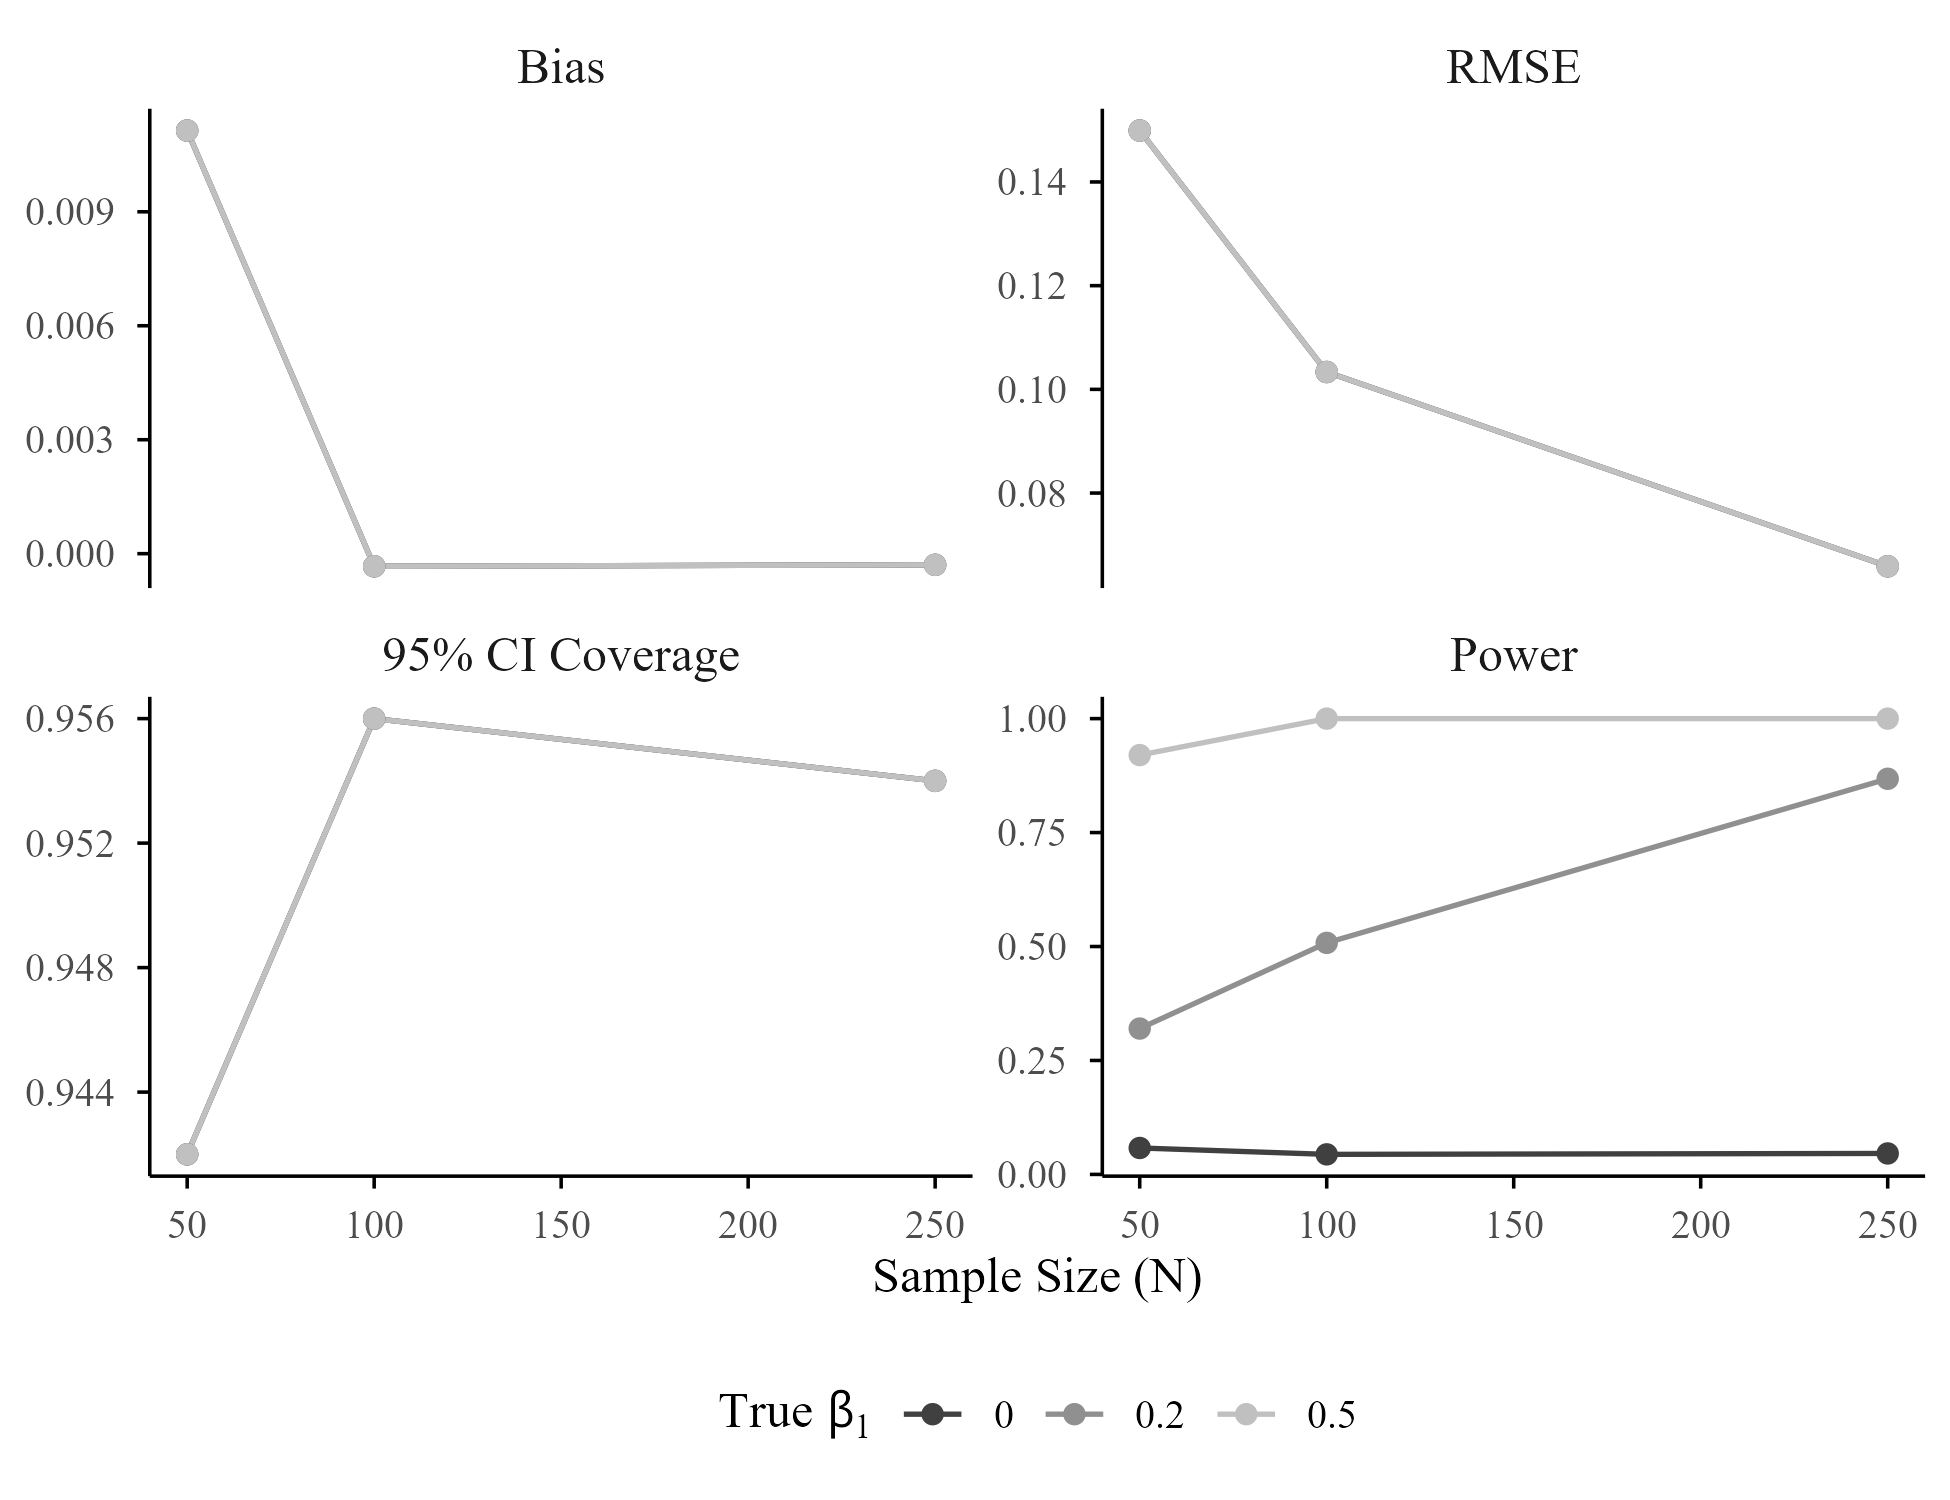
\includegraphics[width=0.9\textwidth]{simulation/figures/fig_sim.png}
  \figurenote{Bias, RMSE, and 95\% CI coverage/power are computed over converged replications only.}
\end{figure}
